\documentclass[11pt,a4paper,twocolumn]{article}

% === Core Packages ===
\usepackage[margin=2cm]{geometry}
\usepackage[utf8]{inputenc}
\usepackage[T1]{fontenc}
\usepackage{times}
\usepackage{amsmath,amssymb}
\usepackage{graphicx}
\usepackage{booktabs}
\usepackage{float}
\usepackage{enumitem}
\usepackage{tikz}
\usepackage{pgfplots}
\pgfplotsset{compat=1.18}
\usetikzlibrary{arrows.meta,shapes.geometric,positioning,calc,decorations.markings,fit,backgrounds}

% === Citation (IEEE style) ===
\usepackage[numbers,sort&compress]{natbib}
\bibliographystyle{IEEEtranN}

% === Hyperref ===
\usepackage[hidelinks]{hyperref}
\usepackage{xurl}

% === Settings ===
\setlength{\parindent}{1em}
\setlength{\parskip}{0.3em}

% === PDF metadata ===
\hypersetup{
  pdftitle={Rete di Reputazione Decentralizzata: Un Quadro per l'Organizzazione Naturale della Società},
  pdfauthor={Pavel Kudrna},
  pdfsubject={Personix — a decentralized reputation network},
  pdfkeywords={Personix, decentralized reputation, reputation social network,
    decentralized identifiers, DID, meritocracy, censorship resistance},
}

% === Title ===
\title{\textbf{Rete di Reputazione Decentralizzata:\\Un Quadro per l'Organizzazione Naturale della Società}}
\author{Pavel Kudrna\\Personix Project --- \url{https://personix.org}\\Prague, Czechia\\Bozza v1 --- Marzo 2026}
\date{}

\begin{document}
\maketitle

% ============================================================
% ABSTRACT
% ============================================================
\begin{abstract}
Il senso di giustizia---la convinzione che i torti vengano riparati e che il merito venga premiato---è la più forte forza coesiva della società. Quando le istituzioni centralizzate di governo non riescono a fornire questo senso perché il costo per far valere un diritto supera il valore del diritto stesso, la coesione sociale si erode. Le attuali strutture istituzionali non riescono a risolvere una classe significativa di controversie sistematicamente nello stesso modo in cui la pianificazione centralizzata non riesce ad allocare le risorse: attraverso l'asimmetria informativa, l'assenza di cicli di feedback e la disconnessione dei decisori dalle conseguenze delle loro decisioni. Questo documento presenta una Rete Sociale di Reputazione (RSN): uno strato di comunicazione decentralizzato, incorruttibile e resistente alla censura, costruito su Identificatori Decentralizzati (DID), che consente a partecipanti pseudonimi di pubblicare, verificare e consumare informazioni reputazionali sul comportamento nel mondo reale. Il meccanismo centrale poggia su tre principi di progettazione: (1)~una struttura di costo asimmetrica in cui leggere i dati reputazionali è poco costoso ma scrivere richiede uno sforzo verificabile; (2)~un protocollo di selezione del verificatore non deterministico basato sull'hashing coerente che pone un prezzo alle affermazioni radicali attraverso costi di iterazione crescenti; e (3)~un modello di autorità reputazionale guidato dal mercato in cui i verificatori privati mettono in gioco la reputazione accumulata sull'accuratezza delle affermazioni che avallano. L'architettura risultante produce una meritocrazia emergente senza coordinamento centrale e consente un percorso di migrazione graduale e reversibile dai sistemi esistenti amministrati dallo Stato.
\end{abstract}

% ============================================================
% 1. INTRODUCTION
% ============================================================
\section{Introduzione}

\subsection{Il Problema della Fiducia Centralizzata}

La governance moderna poggia su un presupposto fondamentale: che le istituzioni centralizzate possano mediare la fiducia tra estranei su larga scala. I tribunali dirimono le controversie. I registri certificano la proprietà. Gli organismi di regolamentazione fanno rispettare gli standard. Queste istituzioni furono concepite in un'epoca in cui l'informazione era scarsa, la comunicazione era lenta e la delega di autorità a un organo centrale era l'unico meccanismo di coordinamento praticabile. La governance centralizzata, tuttavia, fallisce per le stesse ragioni strutturali della pianificazione centralizzata: asimmetria informativa, assenza di cicli di feedback e disconnessione dei decisori dalle conseguenze delle loro decisioni.

Il presupposto fallisce, ad esempio, quando il costo della mediazione istituzionale supera il valore della controversia. Si consideri un inquilino che scopre che l'appartamento in affitto è privo di un certificato di sicurezza elettrica prescritto per legge---una condizione che rappresenta un pericolo immediato per la vita. Il diritto legale dell'inquilino di recedere dal contratto è inequivocabile. Eppure il costo per far valere quel diritto attraverso il sistema giudiziario supera il valore monetario della cauzione e dei danni dovuti, persino includendo un potenziale risarcimento previsto per legge~\cite{czcourtfees}. La risposta razionale è assorbire la perdita e andarsene.

Questo non è un caso limite patologico. È l'esperienza predefinita per una classe significativa di controversie in cui il danno è reale ma la posta economica in gioco scende al di sotto della soglia alla quale l'applicazione istituzionale diventa economicamente razionale. Il risultato è un sistema che favorisce strutturalmente i malintenzionati: coloro che danneggiano gli altri in misura inferiore a questa soglia possono agire impunemente, perché il costo di cercare giustizia ricade sulla parte danneggiata.

L'esempio precedente è tratto dall'ambiente giuridico dell'autore---il sistema di civil law ceco. In altre tradizioni giuridiche---la common law basata sul precedente, il diritto consuetudinario, i sistemi misti---la giustizia fallisce in modi diversi e in gradi diversi, a seconda delle specificità culturali e procedurali della giurisdizione. I lettori probabilmente riconosceranno esempi equivalenti dal proprio contesto. Ciò che è strutturalmente universale è lo schema: le controversie il cui valore scende al di sotto della soglia di applicazione economicamente razionale si concludono con la perdita assorbita dalla parte danneggiata. La RSN non promette una giustizia perfetta---riduce semplicemente il vantaggio strutturale di cui godono i malintenzionati quando l'applicazione istituzionale è antieconomica.

\subsection{Perché le Soluzioni Esistenti Sono Insufficienti}

\textbf{I quadri di Identità Decentralizzata (DID)}~\cite{did2022} forniscono meccanismi crittografici per la gestione dell'identità auto-sovrana, ma si concentrano principalmente sulla verifica dell'identità senza affrontare la questione più ampia della reputazione comportamentale.

\textbf{I Soulbound Token (SBT)}~\cite{weyl2022} colgono l'intuizione che la reputazione non è trasferibile, ma si affidano a un'infrastruttura blockchain con vincoli di scalabilità e non affrontano gli incentivi economici che governano l'inserimento delle informazioni. Concetti correlati come i token di merito (ad es. Liberland) condividono una filosofia simile ma restano legati a quadri giurisdizionali specifici.

\textbf{Le Organizzazioni Autonome Decentralizzate (DAO)}~\cite{buterin2014} attuano la governance attraverso smart contract ma replicano dinamiche plutocratiche in cui l'influenza è proporzionale al capitale. Il voto quadratico~\cite{buterin2019} mitiga in parte questo aspetto ma ne limita l'adozione pratica. Le DAO affrontano inoltre il fondamentale \emph{problema dell'oracolo}: gli smart contract non possono verificare in modo affidabile gli stati del mondo reale senza una fonte esterna fidata, e questo problema non ha una soluzione generale nell'architettura blockchain.

Nessun sistema esistente combina decentralizzazione, resistenza alla censura, pseudonimia, costo di ingresso verificabile e consenso emergente.

\subsection{Contributi}

Questo documento apporta i seguenti contributi:
\begin{enumerate}[nosep]
\item Definizione della \textbf{Rete Sociale di Reputazione (RSN)}, un protocollo decentralizzato che estende il quadro DID per supportare lo scambio bilaterale di reputazione.
\item Un \textbf{protocollo di selezione del verificatore non deterministico} basato sull'hashing coerente~\cite{karger1997}.
\item Il \textbf{Principio del Radicalismo Costoso}, che pone un prezzo alle affermazioni in base alla loro distanza dal consenso della rete attraverso tre canali di costo cumulativi.
\item Un \textbf{modello di Autorità Reputabile} con incentivi asimmetrici in cui un avallo falso costa catastroficamente più delle commissioni legittime.
\item Un \textbf{percorso di migrazione graduale} attraverso un'infrastruttura fiscale parallela.
\end{enumerate}

% ============================================================
% 2. DESIGN PRINCIPLES
% ============================================================
\section{Principi di Progettazione}

L'architettura della RSN è vincolata da cinque principi di progettazione non negoziabili.

\textbf{Continuità ed Evoluzione.} Il sistema coesiste con le istituzioni esistenti durante un periodo di transizione di durata indefinita. La transizione deve essere reversibile in ogni fase.

\textbf{Volontarietà e Responsabilità.} La partecipazione è volontaria, ma la volontarietà è accoppiata alla responsabilità: un partecipante che assume il controllo di una funzione istituzionale assume contemporaneamente gli obblighi che l'accompagnano.

\textbf{Diversità e Neutralità Culturale.} Il consenso emerge dalle interazioni bilaterali, non da regole prestabilite imposte dai progettisti del sistema.

\textbf{Resilienza e Resistenza alla Censura.} Il costo di censurare la rete deve superare il costo di tollerarla. Solo un totalitarismo pieno---a un costo politico ed economico rovinoso---può sopprimere il sistema.

\textbf{Consenso e Applicazione.} Il sistema incorpora le tendenze umane alla meschinità, al dispetto e alla soddisfazione ritorsiva come caratteristiche portanti. La cattiva condotta non è vietata; ha un prezzo.

% ============================================================
% 3. SYSTEM OVERVIEW
% ============================================================
\section{Panoramica del Sistema}

\subsection{Rete Sociale di Reputazione}

La RSN è uno strato di comunicazione decentralizzato, peer-to-peer, in cui i partecipanti scambiano informazioni verificabili sul comportamento nel mondo reale. Le sue proprietà distintive sono: infrastruttura decentralizzata e non censurabile; partecipazione pseudonima tramite DID; struttura di costo asimmetrica (leggere è economico, scrivere è costoso); verificabilità crittografica; e \textbf{supporto agli standard}---formati leggibili dalla macchina per le informazioni propagate attraverso la rete, per i servizi offerti dalle autorità (composizione delle affermazioni, avallo, servizio di testimonianza) e per il formato delle policy, comprese le regole per valutare la reputazione della controparte e valutare il rischio di discrepanza della policy (tra comportamento dichiarato ed effettivo).

\subsection{Componenti Architetturali}

La RSN è costituita da quattro componenti principali (Fig.~\ref{fig:architecture}):
\begin{enumerate}[nosep]
\item \textbf{Strato DID.} Identità dei partecipanti con regole dichiarate, metadati di reputazione e instradamento nella rete.
\item \textbf{Protocollo di Affermazione.} Formato strutturato per pubblicare asserzioni su eventi del mondo reale.
\item \textbf{Rete di Verifica.} Protocollo decentralizzato per assegnare i verificatori usando l'hashing coerente.
\item \textbf{Strato di Aggregazione della Reputazione.} Servizi che producono riepiloghi reputazionali leggibili dall'uomo.
\end{enumerate}

\begin{figure}[ht]
\centering
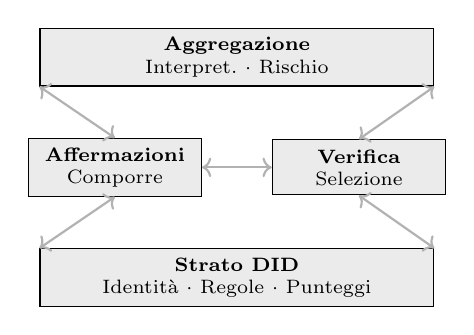
\begin{tikzpicture}[
    layer/.style={draw, minimum height=0.7cm, align=center, font=\scriptsize, fill=black!8},
    arr/.style={<->, thick, gray!60}
]
\node[layer, minimum width=5cm] (agg) at (0,2.8) {\textbf{Aggregazione}\\Interpret.\ $\cdot$ Rischio};
\node[layer, minimum width=2.2cm] (claim) at (-1.55,1.4) {\textbf{Affermazioni}\\Comporre};
\node[layer, minimum width=2.2cm] (verif) at (1.55,1.4) {\textbf{Verifica}\\Selezione};
\node[layer, minimum width=5cm] (did) at (0,0) {\textbf{Strato DID}\\Identità $\cdot$ Regole $\cdot$ Punteggi};

\draw[arr] (agg.south west) -- (claim.north);
\draw[arr] (agg.south east) -- (verif.north);
\draw[arr] (claim.east) -- (verif.west);
\draw[arr] (claim.south) -- (did.north west);
\draw[arr] (verif.south) -- (did.north east);
\end{tikzpicture}
\caption{Architettura a quattro strati della RSN.}
\label{fig:architecture}
\end{figure}

\subsection{Ruoli dei Partecipanti}

Una transazione di verifica coinvolge fino a sei distinti ruoli DID (Fig.~\ref{fig:roles}): \textbf{Emittente} ($DID_I$, crea e sottopone l'affermazione), \textbf{Soggetto} ($DID_S$, il DID a cui l'affermazione si riferisce---può coincidere con l'Emittente), \textbf{Autorità} ($DID_A$, avalla l'affermazione dietro compenso; può anche offrire servizi di testimonianza---\emph{opzionale}), \textbf{Testimone} ($DID_{W_{1..n}}$, monitor in incognito dell'onestà del verificatore tramite codici di sfida---\emph{opzionale}), \textbf{Verificatore} ($DID_V$, selezionato algoritmicamente per pubblicare l'affermazione) e la \textbf{RSN} (la rete in cui vengono pubblicate le affermazioni verificate). Qualsiasi ruolo può essere delegato a un altro DID (Sezione~7.4). Un'Autorità comunemente accorpa l'avallo ai servizi di testimonianza, ma le due funzioni sono logicamente indipendenti.

\begin{figure}[ht]
\centering
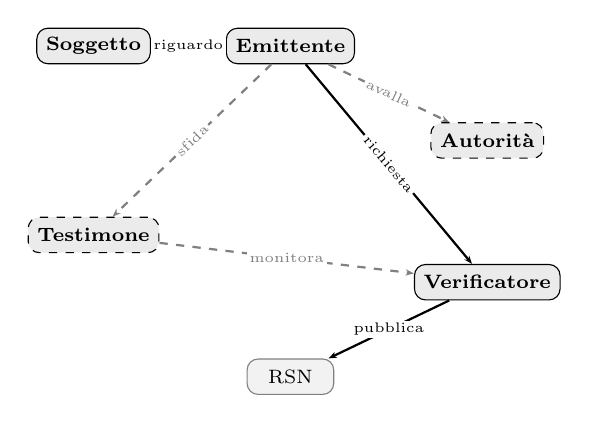
\begin{tikzpicture}[
    role/.style={draw, rounded corners, minimum width=1.1cm, minimum height=0.45cm, align=center, font=\scriptsize, fill=black!8},
    opt/.style={draw, rounded corners, minimum width=1.1cm, minimum height=0.45cm, align=center, font=\scriptsize, fill=black!8, dashed},
    arr/.style={-{Stealth[length=3pt]}, thick},
    oarr/.style={-{Stealth[length=3pt]}, thick, dashed, gray},
    lbl/.style={font=\tiny, fill=white, inner sep=1pt}
]
\node[role] (I) at (0,2.4) {\textbf{Emittente}};
\node[role] (S) at (-2.5,2.4) {\textbf{Soggetto}};
\node[opt] (A) at (2.5,1.2) {\textbf{Autorità}};
\node[opt] (W) at (-2.5,0) {\textbf{Testimone}};
\node[role] (V) at (2.5,-0.6) {\textbf{Verificatore}};
\node[role, fill=black!5, draw=gray] (N) at (0,-1.8) {RSN};

\draw[arr] (I) -- node[lbl] {riguardo} (S);
\draw[oarr] (I) -- node[lbl,sloped] {avalla} (A);
\draw[oarr] (I) -- node[lbl,sloped] {sfida} (W);
\draw[arr] (I) -- node[lbl,sloped] {richiesta} (V);
\draw[oarr] (W) -- node[lbl] {monitora} (V);
\draw[arr] (V) -- node[lbl] {pubblica} (N);
\end{tikzpicture}
\caption{Ruoli DID in una transazione di verifica. Tratteggiato = opzionale (Autorità, Testimone).}
\label{fig:roles}
\end{figure}

\subsection{Incorruttibilità: Quattro Forze}

L'incorruttibilità della RSN non deriva da un singolo meccanismo ma da quattro forze concorrenti. Nessuna è sufficiente da sola; solo la loro combinazione rende economicamente irrazionale un tentativo di corruzione.

\textbf{Bersaglio imprevedibile.} Il verificatore di ogni affermazione è selezionato in modo non deterministico attraverso l'hashing coerente (Sezione~5.3). Un aggressore non può prendere di mira in anticipo un verificatore specifico per corromperlo, perché l'identità del verificatore è una funzione del contenuto dell'affermazione e delle iterazioni precedenti, non della scelta dell'emittente.

\textbf{Leva reputazionale---lenta a salire, rapida a scendere.} La reputazione può essere guadagnata solo in modo incrementale, attraverso un comportamento coerente e sostenuto. Può, tuttavia, essere persa catastroficamente con un singolo avallo fraudolento (Sezione~6.2). Questa asimmetria significa che anni di reputazione accumulata possono essere distrutti da un solo avallo disonesto; la strategia ottimale resta quella di rifiutare le affermazioni sospette.

\textbf{Promessa pubblica.} Ogni Titolare di DID dichiara pubblicamente la propria policy---un insieme di regole leggibili dalla macchina che si impegna a rispettare. La divergenza tra la dichiarazione e il comportamento effettivo è rilevabile e valutata come un'offesa reputazionale più grave della violazione sottostante (Sezione~7.3). L'ipocrisia è quindi più costosa della disonestà diretta.

\textbf{Asimmetria del costo d'attacco della rete a maglia.} Il costo di censurare o destabilizzare la rete cresce in modo non lineare con la dimensione e la densità della rete, mentre il costo di tollerarla resta costante. Perché la censura risulti conveniente, un attore centralizzato dovrebbe applicarla sull'intera rete---richiedendo misure sproporzionate rispetto a qualsiasi beneficio concepibile (Sezione~10).

% ============================================================
% 4. DECENTRALIZED IDENTITY MODEL
% ============================================================
\section{Modello di Identità Decentralizzata}

\subsection{DID con Proprietà Speciali}

La RSN estende la specifica W3C DID Core~\cite{did2022} con: \textbf{Regole Dichiarate} (impegni comportamentali leggibili dalla macchina), \textbf{Metadati di Reputazione} (punteggio comportamentale aggregato) e \textbf{Instradamento nella Rete} (gateway onion mutabile separato dalla posizione stabile nell'anello).

\subsection{Ciclo di Vita dell'Affermazione}

Un'Affermazione procede attraverso sei fasi (Fig.~\ref{fig:lifecycle}): composizione, avallo facoltativo dell'autorità, selezione del verificatore tramite hashing coerente, decisione di verifica (accettazione o rifiuto con iterazione), pubblicazione e aggiornamento della reputazione per tutte le parti.

\begin{figure}[ht]
\centering
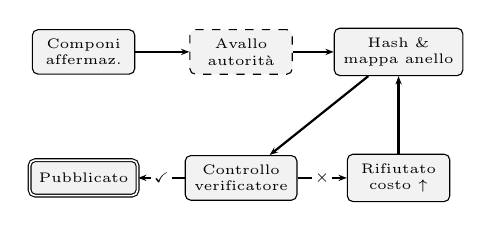
\begin{tikzpicture}[
    stp/.style={draw, rounded corners=2pt, minimum width=1.3cm, minimum height=0.45cm, align=center, font=\tiny, fill=black!5},
    arr/.style={-{Stealth[length=3pt]}, thick},
    lbl/.style={font=\tiny, fill=white, inner sep=1pt}
]
\node[stp] (comp) at (0,0) {Componi\\affermaz.};
\node[stp, dashed] (auth) at (2.0,0) {Avallo\\autorità};
\node[stp] (hash) at (4.0,0) {Hash \&\\mappa anello};
\node[stp] (ver) at (2.0,-1.6) {Controllo\\verificatore};
\node[stp, double] (pub) at (0,-1.6) {Pubblicato};
\node[stp] (rej) at (4.0,-1.6) {Rifiutato\\costo $\uparrow$};

\draw[arr] (comp) -- (auth);
\draw[arr] (auth) -- (hash);
\draw[arr] (hash) -- (ver);
\draw[arr] (ver) -- node[lbl] {\checkmark} (pub);
\draw[arr] (ver) -- node[lbl] {$\times$} (rej);
\draw[arr] (rej) -- ++(0,0.8) -| (hash);
\end{tikzpicture}
\caption{Ciclo di vita dell'affermazione con ciclo di iterazione.}
\label{fig:lifecycle}
\end{figure}

\subsection{Relazione con W3C DID Core}

Il modello di identità della RSN è un sovrainsieme proprio della specifica W3C DID Core~\cite{did2022}. Tutti i DID della RSN sono DID W3C validi. Le estensioni specifiche della RSN sono codificate come proprietà del documento DID definite in una specifica dedicata di metodo DID, compatibile con l'infrastruttura esistente come ION~\cite{buchner2021} e Ceramic~\cite{ceramic2023}.

% ============================================================
% 5. VERIFICATION AND PROPAGATION
% ============================================================
\section{Verifica e Propagazione delle Informazioni}

\subsection{Costo dell'Inserimento delle Informazioni}

Il principio economico centrale della RSN è l'asimmetria tra lettura e scrittura. Leggere i dati reputazionali si avvicina a un costo marginale nullo per i partecipanti che fanno parte della rete DID e hanno un accesso commisurato alla loro reputazione---i nuovi arrivati devono guadagnarsi gradualmente un accesso più ampio (si veda l'anti-parassitismo). Scrivere---inteso come la materializzazione durevole della reputazione nella rete, non come un atto tecnico occasionale---richiede un investimento cumulativo verificabile lungo tre dimensioni: \textbf{tempo} (anni di vita spesi in un comportamento coerente, impegni mantenuti e relazioni coltivate), \textbf{energia} (sforzo investito in rapporti onesti, cura delle collaborazioni e affidabilità a lungo termine) e \textbf{denaro} (investimento nel proprio nome---sviluppo professionale, qualità del proprio lavoro, riparazione dei danni causati). La reputazione non può essere acquistata istantaneamente---è l'esito di un'accumulazione lunga tutta una vita che il sistema si limita a rendere visibile e trasferibile tra contesti. I costi tecnici occasionali del protocollo (firme crittografiche, commissioni dei verificatori) sono trascurabili rispetto a questo investimento di fondo.

\subsection{Grafo Sociale e Profondità dei Contatti}

La RSN è fondamentalmente una rete sociale: ogni DID aggiunge contatti (altri DID) che consentono la connessione. Questi contatti hanno i propri contatti, e così via. La ricerca algoritmica del verificatore opera all'interno di una profondità configurabile $h$ di contatti collegati (ad es. $h=3$: i propri contatti diretti, i loro contatti e i contatti dei contatti). Questa architettura non richiede un'unica blockchain globale---favorisce naturalmente l'emergere di comunità/cluster con sovrapposizioni in altre comunità. Ogni partecipante DID deve avere una \textbf{policy} pubblicata---un insieme di regole leggibili dalla macchina che governa il modo in cui vengono valutate le richieste in arrivo. Le violazioni della policy sono registrate nella rete come artefatti negativi.

\subsection{Selezione Algoritmica del Verificatore}

Il protocollo di verifica impiega l'hashing coerente~\cite{karger1997} (Fig.~\ref{fig:verifier}). La verifica è un servizio a pagamento: i verificatori operano dietro compenso, creando un mercato in cui la concorrenza guida i prezzi, la velocità e l'affidabilità.

\textbf{Passo 1.} Il documento dell'affermazione è concatenato con il risultato hash dell'iterazione precedente (o $\varnothing$ alla prima iterazione) e sottoposto ad hashing:
\begin{equation}
\text{pos} = f_h(\text{claim} \| \text{prev\_hash})
\label{eq:hash}
\end{equation}

L'algoritmo deve includere il \emph{percorso completo} di tutte le richieste e risposte precedenti---non semplicemente un hash dell'iterazione precedente. La risposta completa di ciascun verificatore (accettazione, rifiuto, prezzo indicato, motivazione) viene aggiunta al documento in crescita, verificabile tramite firme crittografiche a ogni passo.

\textbf{Passo 2.} L'hash è mappato su $N$ posizioni sull'anello di hash coerente, distribuite uniformemente (ad es. per $N=4$: $+0^{\circ}, +90^{\circ}, +180^{\circ}, +270^{\circ}$). Da ciascuna posizione, una ricerca in senso orario seleziona il DID più vicino come candidato verificatore (Fig.~\ref{fig:multipoint}). $N$ è un parametro variabile che può dipendere dalla percentuale di DID attualmente attivi, dall'ora del giorno o dalla reattività storica della rete.

\textbf{Passo 3.} Il Verificatore accetta (pubblica, mettendo in gioco la reputazione) o rifiuta (tornando al Passo~1 con l'hash del rifiuto). Quando un nodo non risponde nonostante dichiari uno stato online, la richiesta successiva deve includere tutte le risposte di tutti gli $N$ precedenti candidati verificatori.

\textbf{Anti-parassitismo.} I DID bersaglio possono impostare commissioni o restrizioni di accesso per le interrogazioni provenienti da nuovi DID con poca reputazione. Questo meccanismo graduato (non binario) costringe i nuovi arrivati a costruire reputazione attraverso un'attività genuina prima di consumare liberamente i dati altrui.

\begin{figure}[ht]
\centering
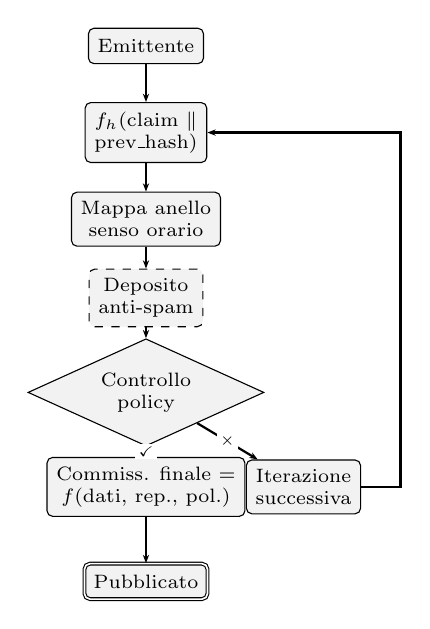
\begin{tikzpicture}[
    box/.style={draw, rounded corners=2pt, minimum width=1.3cm, minimum height=0.45cm, align=center, font=\scriptsize, fill=black!5},
    dec/.style={draw, diamond, aspect=2.2, minimum width=0.9cm, align=center, font=\scriptsize, fill=black!5},
    arr/.style={-{Stealth[length=3pt]}, thick},
    lbl/.style={font=\tiny, fill=white, inner sep=1pt}
]
\node[box] (iss) at (0,0) {Emittente};
\node[box] (hash) at (0,-1.1) {$f_h$(claim $\|$\\prev\_hash)};
\node[box] (ring) at (0,-2.2) {Mappa anello\\senso orario};
\node[box, dashed] (spam) at (0,-3.2) {Deposito\\anti-spam};
\node[dec] (check) at (0,-4.4) {Controllo\\policy};
\node[box] (rej) at (2,-5.6) {Iterazione\\successiva};
\node[box] (fee) at (0,-5.6) {Commiss. finale =\\$f$(dati, rep., pol.)};
\node[box, double] (pub) at (0,-6.8) {Pubblicato};

\draw[arr] (iss) -- (hash);
\draw[arr] (hash) -- (ring);
\draw[arr] (ring) -- (spam);
\draw[arr] (spam) -- (check);
\draw[arr] (check) -- node[lbl] {$\times$} (rej);
\draw[arr] (check) -- node[lbl] {\checkmark} (fee);
\draw[arr] (fee) -- (pub);
\draw[arr] (rej.east) -- ++(0.5,0) |- (hash.east);
\end{tikzpicture}
\caption{Protocollo di selezione del verificatore. Il deposito anti-spam è opzionale e può essere rimborsabile. La commissione finale è pagata solo in caso di accettazione.}
\label{fig:verifier}
\end{figure}

Ogni rifiuto aggiunge la risposta completa del verificatore (comprese motivazioni e condizioni) al documento dell'affermazione, ampliandone il contenuto. Dal documento ampliato viene calcolato in modo non deterministico un nuovo hash, che si mappa su una diversa posizione dell'anello e seleziona un verificatore differente. La documentazione del percorso completo è obbligatoria---l'emittente non può prevedere né influenzare il verificatore successivo. Se un verificatore ignora una richiesta nonostante una policy dichiarata compatibile, i testimoni (se presenti) lo registrano, e l'emittente può allegare le prove testimoniali al momento della pubblicazione finale.

\begin{figure}[ht]
\centering
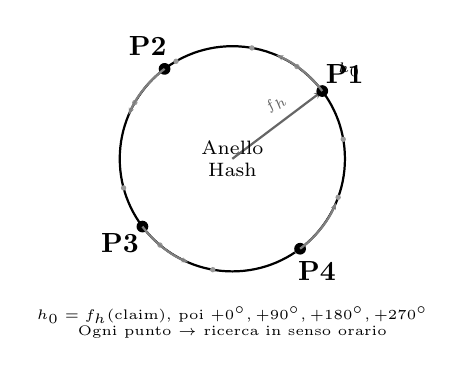
\begin{tikzpicture}[scale=0.65]
% Ring
\draw[thick] (0,0) circle (2.2cm);
% DID nodes on ring
\foreach \a in {10,55,80,120,150,195,230,260,305,340} {
  \fill[black!40] (\a:2.2) circle (1.5pt);
}
% Hash offset arrow pointing to initial position
\draw[-{Stealth[length=3pt]}, thick, black!60] (0,0) -- node[font=\tiny,above,sloped,pos=0.6] {$f_h$} (37:2.2);
\fill[black] (37:2.2) circle (2pt);
\node[font=\tiny,anchor=south west] at (37:2.35) {$h_0$};
% N=4 points offset from h0 by +0, +90, +180, +270
\foreach \offset/\l in {0/P1,90/P2,180/P3,270/P4} {
  \pgfmathsetmacro{\ang}{37+\offset}
  \node[fill=black, circle, inner sep=1.5pt] (p\offset) at (\ang:2.2) {};
  \node[font=\tiny,font=\bfseries] at (\ang:2.75) {\l};
  % clockwise search arc
  \draw[-{Stealth[length=2.5pt]}, thick, gray] (\ang:2.2) arc (\ang:\ang+30:2.2);
}
\node[font=\scriptsize, align=center] at (0,0) {Anello\\Hash};
\node[font=\tiny, align=center] at (0,-3.2) {$h_0 = f_h(\text{claim})$, poi $+0^{\circ},+90^{\circ},+180^{\circ},+270^{\circ}$\\Ogni punto $\rightarrow$ ricerca in senso orario};
\end{tikzpicture}
\caption{Selezione multi-punto ($N{=}4$). L'hash $h_0$ imposta l'offset; 4 punti distribuiti uniformemente da $h_0$.}
\label{fig:multipoint}
\end{figure}

\subsection{Protocollo del Testimone}

Il ruolo del \textbf{Testimone} fornisce responsabilità in incognito per l'onestà del verificatore attraverso un protocollo crittografico di codici di sfida:

\textbf{Passo W1.} Il richiedente firma la richiesta di verifica e la invia a $N_w$ testimoni---contatti della rete sociale del richiedente, o fornitori specializzati di servizi di testimonianza operanti dietro compenso.

\textbf{Passo W2.} Ogni testimone $w_i$ firma l'intera richiesta firmata, conserva la firma originale $\sigma_i$ e calcola un codice di sfida $c_i = h(\sigma_i)$. Il codice di sfida viene aggiunto alla richiesta.

\textbf{Passo W3.} La richiesta, che ora reca $N_w$ codici di sfida, viene inviata al verificatore. Il verificatore osserva i codici ma \emph{non può determinare} chi siano i testimoni né se i codici corrispondano a firme reali.

\textbf{Passo W4 (verificatore onesto).} Se il verificatore risponde secondo la policy dichiarata, i codici di sfida restano opachi. I testimoni non vengono mai rivelati. Non vengono pubblicati dati aggiuntivi.

\textbf{Passo W5 (violazione della policy).} Se il verificatore viola la propria policy (ignora la richiesta, risponde in modo incoerente), il richiedente detiene le firme originali dei testimoni $\sigma_i$. Queste possono essere pubblicate come dati di accompagnamento: chiunque può verificare $c_i = h(\sigma_i)$, dimostrando che il testimone era presente. Il richiedente può pubblicare in modo indipendente---il verificatore ha già firmato i codici di sfida nella propria risposta.

\textbf{La proprietà del bluff.} Il richiedente può sostituire valori casuali ad alcuni o a tutti i codici di sfida. Il verificatore non può distinguere i codici genuini (sostenuti da autorità ad alta reputazione) dal rumore. Questa \emph{incertezza} è il meccanismo di applicazione: ogni richiesta comporta il rischio che un'autorità rispettata stia osservando in incognito. Il costo di mantenere questa pressione è prossimo allo zero (generare numeri casuali), mentre il potenziale costo della disonestà per il verificatore è catastrofico. Il comportamento onesto è incentivato anche in assenza di testimoni effettivi.

\textbf{Autorità come testimone.} Un'Autorità che avalla un'affermazione può accorpare i servizi di testimonianza: ``Avallo la tua affermazione e fungo da testimone in incognito durante la verifica.'' Questo è un modello di business naturale---l'Autorità dispone già del contesto. Tuttavia, i due ruoli sono logicamente indipendenti.

\subsection{Principio del Radicalismo Costoso}

Tre canali di costo si sommano simultaneamente (Fig.~\ref{fig:radicalism}):

\textbf{Canale 1: Costo di Iterazione.} Ogni rifiuto impone una nuova iterazione che consuma tempo e risorse. Crescita lineare.

\textbf{Canale 2: Gonfiamento del Documento.} Ogni iterazione aggiunge la risposta completa del verificatore al documento dell'affermazione. La crescita è lineare, ma con un offset di base: il carico iniziale (contenuto dell'affermazione, avallo dell'autorità, firme crittografiche) ha già una dimensione non trascurabile $B_0$. Dimensione totale dopo $k$ iterazioni: $S(k) = B_0 + k \cdot \Delta$, dove $\Delta$ è la dimensione media della risposta.

\textbf{Canale 3: Premio di Rischio del Verificatore.} Il rischio è soggettivo. Il verificatore valuta se le policy dichiarate del DID richiedente confliggano con i propri interessi commerciali, sociali o politici. Il premio può crescere in modo esponenziale con la distanza percepita dall'``ideale'' del verificatore: $P(d) = \alpha \cdot e^{\beta d}$, dove $d$ è la metrica soggettiva di distanza del verificatore. Oltre un confine personale invalicabile, il verificatore può rifiutare del tutto.

\begin{figure}[ht]
\centering
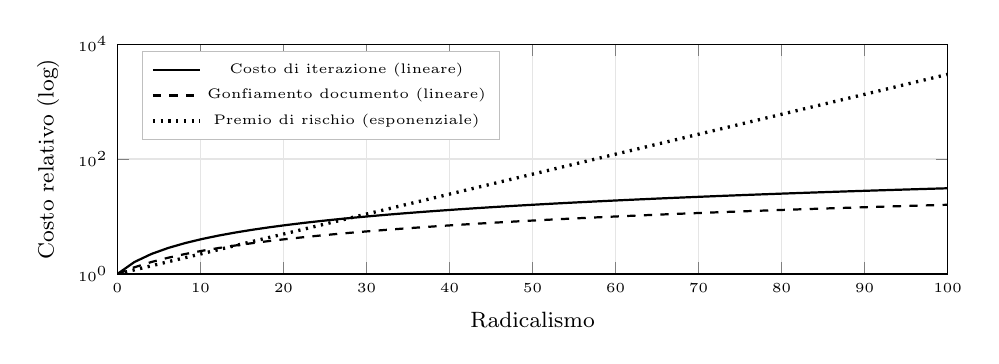
\begin{tikzpicture}
\begin{axis}[
    width=\columnwidth,
    height=4.5cm,
    xlabel={\footnotesize Radicalismo},
    ylabel={\footnotesize Costo relativo (log)},
    ymode=log,
    xmin=0, xmax=100,
    ymin=1, ymax=10000,
    grid=major,
    grid style={gray!20},
    legend style={at={(0.03,0.97)},anchor=north west,font=\tiny,draw=gray!50},
    tick label style={font=\tiny},
    label style={font=\footnotesize},
]
\addplot[black, thick, domain=0:100, samples=50] {1 + 0.3*x};
\addlegendentry{Costo di iterazione (lineare)}
\addplot[black, thick, dashed, domain=0:100, samples=50] {1 + 0.15*x};
\addlegendentry{Gonfiamento documento (lineare)}
\addplot[black, thick, dotted, line width=1.2pt, domain=0:100, samples=100] {exp(0.08*x)};
\addlegendentry{Premio di rischio (esponenziale)}
\end{axis}
\end{tikzpicture}
\caption{Escalation dei costi attraverso tre canali. Il premio di rischio domina in condizioni di alto radicalismo.}
\label{fig:radicalism}
\end{figure}

Fondamentalmente, questa non è censura. Nessuna affermazione è vietata. Il sistema pone un prezzo al rischio (Tabella~\ref{tab:costs}).

\begin{table}[ht]
\centering
\caption{Confronto dei costi tra i tipi di affermazione.}
\label{tab:costs}
\footnotesize
\begin{tabular}{@{}lcccc@{}}
\toprule
\textbf{Tipo} & \textbf{Iter.} & \textbf{Doc} & \textbf{Comm.} & \textbf{Totale} \\
\midrule
Credibile & $k_{\min}$ & $B_0$ & $P_{\min}$ & Basso \\
Controversa & $k_{\text{med}}$ & $B_0{+}k\Delta$ & $\alpha e^{\beta d}$ & Moderato \\
Radicale & $k_{\max}$ & $\gg B_0$ & $\gg P_{\min}$ & Molto alto \\
Fraudolenta & $\to\infty$ & --- & --- & Impubblicabile \\
\bottomrule
\end{tabular}
\end{table}

% ============================================================
% 6. REPUTATION AND RISK
% ============================================================
\section{Reputazione e Valutazione del Rischio}

\subsection{Modello di Accumulazione della Reputazione}

La reputazione presenta tre proprietà: \textbf{accumulazione lenta} (crescita incrementale attraverso un comportamento coerente), \textbf{distruzione rapida} (una singola frode può ridurre catastroficamente il punteggio) e \textbf{valutazione individuale} (ogni parte consumatrice può applicare la propria funzione di aggregazione).

\subsection{Autorità Reputabili}

Un'Autorità Reputabile esamina le affermazioni e, se soddisfatta, le controfirma---mettendo in gioco la propria reputazione (Fig.~\ref{fig:authority}). L'asimmetria è voluta per progetto: guadagnare reputazione è lento (incremento $+\delta$ per ogni avallo onesto), mentre perderla è catastrofico ($-\Delta \gg \delta$ per ogni avallo falso; a titolo illustrativo, ad es. $+2\%$ contro $-70\%$). La strategia ottimale è sempre rifiutare le affermazioni sospette. I valori specifici di $\delta$ e $\Delta$ sono parametri del sistema.

\begin{figure}[ht]
\centering
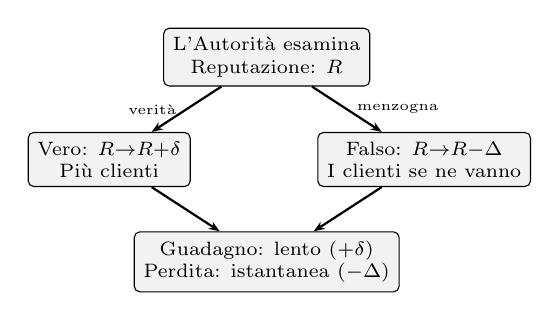
\begin{tikzpicture}[
    box/.style={draw, rounded corners=2pt, minimum width=2cm, minimum height=0.6cm, align=center, font=\scriptsize, fill=black!5},
    arr/.style={-{Stealth[length=4pt]}, thick}
]
\node[box] (exam) at (0,0) {L'Autorità esamina\\Reputazione: $R$};
\node[box] (true) at (-2,-1.3) {Vero: $R{\to}R{+}\delta$\\Più clienti};
\node[box] (false) at (2,-1.3) {Falso: $R{\to}R{-}\Delta$\\I clienti se ne vanno};
\node[box] (insight) at (0,-2.6) {Guadagno: lento ($+\delta$)\\Perdita: istantanea ($-\Delta$)};

\draw[arr] (exam) -- node[left,font=\tiny] {verità} (true);
\draw[arr] (exam) -- node[right,font=\tiny] {menzogna} (false);
\draw[arr] (true) -- (insight);
\draw[arr] (false) -- (insight);
\end{tikzpicture}
\caption{Autorità Reputabile---incentivi asimmetrici.}
\label{fig:authority}
\end{figure}

\subsection{Reputazione Multidimensionale}

La reputazione non è uno scalare ma un vettore lungo più dimensioni: affidabilità finanziaria, integrità personale, competenza professionale, impegno civico e altre (Fig.~\ref{fig:reputation-radar}). Fornitori di valutazione diversi proiettano questo vettore in modi diversi a seconda del contesto---un finanziatore dà priorità all'affidabilità finanziaria, un datore di lavoro alla competenza professionale, un vicino al comportamento civico. Non esiste un unico punteggio di reputazione ``corretto''; solo prospettive.

\begin{figure}[ht]
\centering
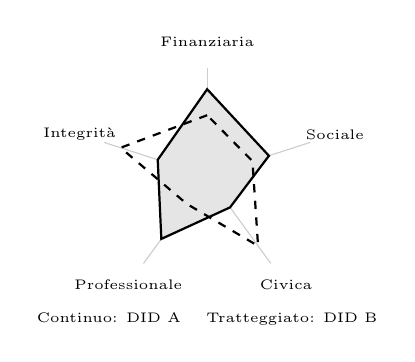
\begin{tikzpicture}[scale=0.55]
\foreach \a/\l in {90/Finanziaria,162/Integrità,234/Professionale,306/Civica,18/Sociale} {
  \draw[gray!40] (0,0) -- (\a:2.5);
  \node[font=\tiny, align=center] at (\a:3.1) {\l};
  \foreach \r in {0.8,1.6,2.4} {
    \fill[black!15] (\a:\r) circle (0.5pt);
  }
}
\draw[thick, fill=black!10] (90:2.0) -- (162:1.2) -- (234:1.8) -- (306:0.9) -- (18:1.5) -- cycle;
\draw[thick, dashed] (90:1.4) -- (162:2.1) -- (234:0.8) -- (306:2.0) -- (18:1.1) -- cycle;
\node[font=\tiny] at (0,-3.3) {Continuo: DID A \quad Tratteggiato: DID B};
\end{tikzpicture}
\caption{Vettori di reputazione multidimensionali. DID diversi mostrano profili diversi lungo le dimensioni.}
\label{fig:reputation-radar}
\end{figure}

\subsection{Valutazione del Rischio Democratizzata}

La RSN democratizza la valutazione sistematica del rischio---una capacità attualmente concentrata nelle istituzioni finanziarie ma applicabile ben oltre il settore bancario. Conglomerati industriali che valutano l'affidabilità dei fornitori, compagnie assicurative che prezzano il rischio comportamentale, due diligence per fusioni e acquisizioni, stima della durata delle attrezzature nella produzione manifatturiera---ovunque il rischio di controparte richieda una valutazione, la RSN offre un'alternativa decentralizzata e guidata dal mercato. Un mercato di servizi di interpretazione traduce i dati grezzi di reputazione multidimensionale in riepiloghi utilizzabili, rendendo la valutazione della controparte accessibile a qualsiasi partecipante a un costo marginale.

% ============================================================
% 7. CONSENSUS AND DISPUTE RESOLUTION
% ============================================================
\section{Consenso e Risoluzione delle Controversie}

\subsection{Modello di Giustizia Decentralizzata}

La RSN riformula la giustizia come un problema di negoziazione bilaterale. La minaccia di un danno reputazionale permanente e verificabile è un deterrente più efficace dei procedimenti legali che la parte danneggiata non può permettersi.

\subsection{Consenso Emergente}

Ogni partecipante mantiene una soglia personale di soddisfazione. Il consenso aggregato della rete emerge come media statistica di migliaia di negoziazioni bilaterali (Fig.~\ref{fig:consensus}). Una risposta molto al di sopra del consenso (barbarica) è costosa da pubblicare. Una risposta vicina al consenso (proporzionale) è economica. Il consenso non è una regola---è un segnale di prezzo.

\begin{figure}[ht]
\centering
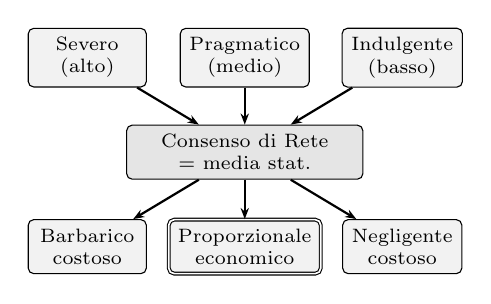
\begin{tikzpicture}[
    person/.style={draw, rounded corners=2pt, minimum width=1.5cm, minimum height=0.5cm, align=center, font=\scriptsize, fill=black!5},
    arr/.style={-{Stealth[length=4pt]}, thick}
]
\node[person] (a) at (-2,0) {Severo\\(alto)};
\node[person] (b) at (0,0) {Pragmatico\\(medio)};
\node[person] (c) at (2,0) {Indulgente\\(basso)};
\node[person, fill=black!10, minimum width=3cm] (cons) at (0,-1.2) {Consenso di Rete\\= media stat.};
\node[person] (exp) at (-2,-2.4) {Barbarico\\costoso};
\node[person, double] (prop) at (0,-2.4) {Proporzionale\\economico};
\node[person] (neg) at (2,-2.4) {Negligente\\costoso};

\draw[arr] (a) -- (cons);
\draw[arr] (b) -- (cons);
\draw[arr] (c) -- (cons);
\draw[arr] (cons) -- (exp);
\draw[arr] (cons) -- (prop);
\draw[arr] (cons) -- (neg);
\end{tikzpicture}
\caption{Consenso emergente dalle soglie individuali di soddisfazione.}
\label{fig:consensus}
\end{figure}

\subsection{Calibrazione della Punizione}

Ogni Titolare di DID dichiara pubblicamente le risposte a specifiche categorie di cattiva condotta. Dichiarazioni sproporzionatamente dure o indulgenti attirano segnali reputazionali negativi. Le dichiarazioni proporzionali sono accettate senza attriti---un sistema di punizione auto-calibrante.

Le dichiarazioni di consenso sono a loro volta soggette al rilevamento dell'ipocrisia: impegnarsi dichiarativamente su una posizione di consenso comportandosi in modo incoerente costituisce un'offesa reputazionale più grave della deviazione sottostante, poiché dimostra un inganno intenzionale.

\subsection{Delega}

Tutte le attività all'interno di un DID---con un'eccezione---possono essere delegate a un altro DID. \textbf{Il ruolo di Soggetto---il DID a cui si riferisce il comportamento oggetto dell'affermazione---non può essere delegato; è legato in modo non trasferibile al titolare dell'identità a cui l'affermazione si riferisce.} Gli altri ruoli attivi---Emittente, Autorità, Testimone, Verificatore---possono essere trasferiti a un DID delegato designato, sia per la verifica, la sottomissione di affermazioni, la partecipazione al consenso o la risoluzione delle controversie. La delega è revocabile in qualsiasi momento. Ciò consente la specializzazione (ad es. servizi professionali di verifica) mentre il Titolare mantiene il controllo e la responsabilità ultimi. La delega si applica all'intero sistema ed è essenziale per la scalabilità.

\subsection{Dalla Moralità Individuale al Contratto Sociale Emergente}

La policy dichiarata di ogni DID rappresenta una formalizzazione della moralità individuale: ciò che il Titolare considera accettabile, come risponde a comportamenti specifici, cosa richiede dalle controparti. Queste policy non sono imposte da un progettista di sistema---sono scelte da ciascun partecipante ed espresse in forma leggibile dalla macchina.

Questa formalizzazione consente un'emergenza in tre fasi. Primo, la moralità individuale è codificata come \textbf{policy}---un insieme di regole dichiarate, soglie e funzioni di risposta che il DID si impegna a rispettare. Secondo, l'aggregato di tutte le policy attraverso la rete produce un'\textbf{etica emergente}---norme statisticamente osservabili che nessun singolo partecipante ha progettato ma che sorgono dall'interazione di migliaia di posizioni morali individuali~\cite{durkheim1893}. Terzo, questa etica emergente, espressa come norme comportamentali condivise applicate attraverso segnali di prezzo bilaterali, costituisce un \textbf{contratto sociale misurabile}---non un costrutto teorico che nessuno ha firmato~\cite{rawls1971}, ma un insieme di regole empiricamente osservabile e sostenuto dal comportamento effettivo.

Questo processo rispecchia i risultati della teoria dei fondamenti morali~\cite{haidt2012}: la moralità umana è intuitiva, pluralistica e culturalmente variabile. La RSN non richiede un consenso morale come input; produce un consenso comportamentale come output. Il contratto sociale risultante non è statico---evolve man mano che i partecipanti entrano, escono e adattano le proprie policy in risposta al feedback della rete. A differenza della teoria classica del contratto sociale, questo contratto è revocabile, osservabile e applicabile senza un sovrano.

% ============================================================
% 8. ECONOMIC MODEL
% ============================================================
\section{Modello Economico}

Le sezioni precedenti hanno descritto uno strumento---i meccanismi di verifica della RSN, la struttura dei costi e il consenso emergente. Questa sezione descrive una metodologia per applicare tale strumento alla transizione fiscale e di governance. Lo strumento è di uso generale; la metodologia sottostante è una possibile applicazione.

\subsection{Struttura degli Incentivi}

La reputazione come capitale crea incentivi diretti al comportamento onesto. In condizioni normali di funzionamento, i partecipanti costruiscono reputazione naturalmente attraverso le transazioni quotidiane e gli impegni mantenuti. La spesa principale riguarda le affermazioni \emph{negative}---la registrazione del danno arrecato da altri. Questa asimmetria incentiva un comportamento utile e affidabile: essere onesti non costa nulla in più, mentre essere dannosi crea una traccia documentata che altri saranno disposti a pagare per preservare. L'ipocrisia---dichiarare regole senza seguirle---è la modalità di fallimento più costosa, poiché dimostra un inganno intenzionale.

\subsection{Sistema Fiscale Parallelo}

Tre componenti abilitano una pressione competitiva: (1)~\textbf{Imposta Semplice}---un'unica aliquota proporzionale senza eccezioni, inizialmente marginalmente al di sotto dell'aliquota effettiva esistente; (2)~\textbf{Registrazione Elettronica della Spesa (ESR)}---che inverte il modello ceco EET affinché i cittadini sorveglino le spese dello Stato; (3)~\textbf{Allocazione Fiscale Diretta dei Cittadini}---che parte da una manciata di punti percentuali nel primo anno e raggiunge, dopo un decennio, dalle basse decine di punti percentuali fino a una migrazione completa verso un sistema diretto dai cittadini, a seconda del ritmo di adozione. Il tempo effettivo dipende dalla velocità con cui emergono alternative di libero mercato ai servizi statali e dalla disponibilità dello Stato a cooperare alla transizione; la funzione del tempo non deve necessariamente essere lineare, e non c'è ragione di fissare un limite superiore al punto in cui l'adozione può infine arrivare.

% ============================================================
% 9. MIGRATION PATH
% ============================================================
\section{Percorso di Migrazione}

La migrazione procede attraverso tre fasi (Fig.~\ref{fig:migration}): \textbf{Fase~1: Sovrapposizione} (RSN come strato informativo, lo Stato è l'unico fornitore), \textbf{Fase~2: Concorrenza} (RSN fornisce alternative funzionali, uso a doppio sistema) e \textbf{Fase~3: Transizione} (RSN supera gli equivalenti statali, migrazione volontaria). La transizione è reversibile in ogni fase.

\begin{figure}[ht]
\centering
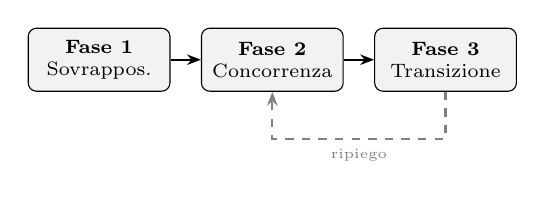
\begin{tikzpicture}[
    phase/.style={draw, rounded corners=3pt, minimum width=1.8cm, minimum height=0.8cm, align=center, font=\scriptsize, fill=black!5},
    arr/.style={-{Stealth[length=5pt]}, thick}
]
\node[phase] (p1) at (0,0) {\textbf{Fase 1}\\Sovrappos.};
\node[phase] (p2) at (2.2,0) {\textbf{Fase 2}\\Concorrenza};
\node[phase] (p3) at (4.4,0) {\textbf{Fase 3}\\Transizione};

\draw[arr] (p1) -- (p2);
\draw[arr] (p2) -- (p3);
\draw[arr, dashed, gray] (p3.south) -- ++(0,-0.6) -| node[below,font=\tiny,pos=0.25] {ripiego} (p2.south);
\end{tikzpicture}
\caption{Migrazione in tre fasi---reversibile in ogni fase.}
\label{fig:migration}
\end{figure}

Il principale meccanismo di pressione è fiscale: quando i contribuenti condizionali raggiungono una ``minoranza economicamente significativa $X$''---un gruppo abbastanza grande da rendere la repressione contro di esso causa di danni economici non trascurabili e da rendere la disobbedienza civile una minaccia credibile---lo Stato entra in negoziazione. A titolo illustrativo, usiamo $X \approx 15\%$ del PIL, ma la soglia effettiva dipende dalla specifica economia.

% ============================================================
% 10. SECURITY ANALYSIS
% ============================================================
\section{Analisi della Sicurezza}

Consideriamo cinque categorie di avversari: singoli malintenzionati, gruppi organizzati, avversari aziendali, avversari a livello statale e avversari a livello di protocollo.

\textbf{Resistenza Sybil}~\cite{douceur2002}. Costruire reputazione richiede un'interazione sostenuta e verificabile. Il costo di un attacco Sybil riuscito cresce linearmente con le identità false e quadraticamente con il livello di reputazione bersaglio. Operare più DID in parallelo è possibile ma costoso per progetto---ogni identità deve accumulare reputazione in modo indipendente attraverso un'attività genuina. Nelle società libere questo costo scoraggia l'abuso occasionale; nelle dittature, i DID paralleli diventano uno strumento di sopravvivenza che consente resistenza compartimentata, coordinamento clandestino e una navigazione più sicura del mercato nero.

\textbf{Difesa dalla collusione.} Gli schemi di avallo reciproco tra gruppi chiusi sono rilevabili attraverso l'analisi del grafo sociale. Le funzioni di aggregazione della reputazione scontano le affermazioni provenienti da fonti strettamente raggruppate.

\textbf{Avversario a livello statale.} L'instradamento onion, l'assenza di infrastruttura centralizzata e la distribuzione del ruolo di Verificatore tra la base dei partecipanti assicurano che la soppressione richieda misure sproporzionate rispetto a qualsiasi beneficio.

\textbf{Privacy contro responsabilità.} La pseudonimia---una via di mezzo tra l'anonimato e la divulgazione dell'identità---consente ai DID di accumulare reputazione significativa senza rivelare l'identità reale del Titolare.

% ============================================================
% 11. PRIVACY
% ============================================================
\section{Considerazioni sulla Privacy}

Il modello di privacy della RSN è costruito sulla pseudonimia. Il Titolare controlla la divulgazione dell'identità: minima (pseudonimo puro), selettiva (credenziali specifiche collegate) o completa (identità legale associata). Le affermazioni pubblicate sono permanenti---il sistema supporta la correzione contestuale ma non la cancellazione. Un Titolare può abbandonare un DID compromesso e ricominciare da capo, rinunciando alla reputazione accumulata.

% ============================================================
% 12. RELATED WORK
% ============================================================
\section{Lavori Correlati}

La specifica W3C DID Core~\cite{did2022} e la Ceramic Network~\cite{ceramic2023} forniscono la base identitaria. EigenTrust~\cite{kamvar2003} ha dimostrato l'aggregazione distribuita della reputazione senza un'autorità centrale. Gli SBT~\cite{weyl2022} hanno introdotto i token sociali non trasferibili. La RSN si distingue per l'enfasi sul costo economico come filtro di qualità e per il suo meccanismo di prezzatura del radicalismo.

Le DAO~\cite{buterin2014} e il voto quadratico~\cite{buterin2019} hanno dimostrato la fattibilità della governance decentralizzata. La RSN deriva il consenso dalle negoziazioni bilaterali sui prezzi anziché dal voto.

La proposta attinge alla teoria anarco-capitalista~\cite{rothbard1973,hoppe2001} per la fornitura privata di servizi ma se ne discosta in due aspetti critici: progetta per il dispetto e gli impulsi ritorsivi anziché presumere la razionalità, e propone una transizione graduale anziché una rivoluzione. Il concetto di contratti sociali emergenti ha precedenti nella teoria hayekiana dell'ordine spontaneo~\cite{hayek1973}.

\textbf{Anarco-agorismo.} La RSN condivide un significativo terreno comune con la contro-economia agorista~\cite{konkin2006}---in particolare l'enfasi sulla costruzione di istituzioni parallele e sullo scambio volontario. Tuttavia, l'agorismo tende a presumere l'interesse personale razionale come meccanismo di coordinamento sufficiente e spesso manca di un percorso concreto di migrazione dalle strutture statali esistenti. La RSN incorpora esplicitamente tendenze comportamentali non razionali e fornisce un meccanismo di pressione fiscale per una transizione graduale.

\textbf{Meritocrazia.} La RSN potrebbe rappresentare una prima descrizione funzionale di come la meritocrazia~\cite{young1958} possa emergere come proprietà sistemica anziché come slogan. I sistemi meritocratici tradizionali falliscono perché richiedono un'autorità centrale per definire e far rispettare il ``merito''. Nella RSN, il merito emerge dalle valutazioni bilaterali: chi genera valore accumula reputazione; nessun comitato decide chi ha merito.

\textbf{La proprietà come privilegio.} La RSN si discosta fondamentalmente dalle trattazioni anarco-capitaliste e della scuola austriaca dei diritti di proprietà come naturali e assoluti. Nel quadro della RSN, la proprietà è un \emph{privilegio}---un riconoscimento sociale che può, in casi estremi, essere revocato dalla comunità quando un partecipante viola fondamentalmente le norme condivise (tradimento, rifiuto di difendere la comunità in una crisi esistenziale, sfruttamento sistematico). Questa non è un'espropriazione statale ma un ritiro del riconoscimento sociale da parte della rete di relazioni bilaterali.

% ============================================================
% 13. LIMITATIONS
% ============================================================
\section{Discussione e Limitazioni}

\textbf{Avvio a freddo.} Il valore della RSN dipende dagli effetti di rete; i primi adottanti affrontano un valore limitato finché la partecipazione non raggiunge una soglia. Tuttavia, anche dalle fasi iniziali, la rete DID funge da utile fonte informativa supplementare. La valutazione precoce della reputazione e delle autorità è destinata a svilupparsi gradualmente con crescente sofisticazione.

\textbf{Anti-parassitismo e controllo dell'accesso.} I DID bersaglio possono imporre commissioni graduate e restrizioni di accesso alle interrogazioni provenienti da DID a bassa reputazione. Questa non è una scala binaria ma continua: meno reputazione ha un DID interrogante, meno informazioni riceve, più a lungo attende e più paga. Questo meccanismo incentiva una partecipazione genuina rispetto al consumo passivo.

\textbf{Disuguaglianza di accesso.} Il costo di pubblicare affermazioni potrebbe filtrare le rimostranze legittime dei partecipanti economicamente svantaggiati. Mitigazione: ogni partecipante funge simultaneamente da potenziale verificatore (o delega questo ruolo) e guadagna commissioni di verifica. Su un orizzonte temporale sufficiente, un partecipante non radicale dovrebbe avvicinarsi alla neutralità finanziaria---i proventi della verifica che compensano approssimativamente i costi di pubblicazione. Questa è un'aspettativa statistica, non una garanzia.

\textbf{Disuguaglianza reputazionale.} I primi adottanti accumulano vantaggi che possono creare barriere per chi arriva più tardi. Tuttavia, la valutazione della reputazione è eseguita da fornitori terzi che possono scegliere di mitigare il vantaggio del primo entrante attraverso i propri algoritmi di aggregazione. Essere i primi con una buona reputazione è un legittimo vantaggio economico comparativo---e questo è voluto per progetto.

\textbf{Questioni aperte.} Le funzioni di costo ottimali, gli standard di aggregazione, la governance del protocollo e l'interazione con i dati reputazionali sintetici generati dall'IA restano aree per lavori futuri.

Questo documento non sostiene che la RSN produrrà risultati ottimali in ogni circostanza. Sostiene che la RSN rappresenta un'alternativa \emph{fattibile}---tecnicamente implementabile, economicamente autosufficiente e socialmente compatibile con le tendenze comportamentali umane così come sono realmente.

% ============================================================
% 14. CONCLUSION
% ============================================================
\section{Conclusione}

Questo documento ha presentato la Rete Sociale di Reputazione, un protocollo decentralizzato che consente uno scambio di reputazione pseudonimo e verificabile. Il Principio del Radicalismo Costoso assicura che le affermazioni fraudolente siano escluse dal prezzo senza censura. Il percorso di migrazione proposto consente una transizione graduale e reversibile dalle istituzioni esistenti. La progettazione incorpora la natura umana così com'è---compresi la meschinità, il dispetto e il desiderio di soddisfazione ritorsiva---anziché richiedere una trasformazione ideologica. Il risultato non è un'utopia ma un sistema in cui la giustizia è accessibile, la reputazione è guadagnata e il costo della cattiva condotta è sostenuto dalla parte che l'ha causata.

% ============================================================
% REFERENCES
% ============================================================
\bibliography{references}

\end{document}
